\documentclass[11pt]{article}
\usepackage[pdfborder={0 0 0}]{hyperref}
\usepackage[english]{babel}
\usepackage{listings}
\usepackage{color}
\usepackage{graphicx}
\usepackage{epstopdf}
\usepackage{multirow}
\setlength{\parskip}{\baselineskip}

\definecolor{codegreen}{rgb}{0,0.6,0}
\definecolor{codegray}{rgb}{0.5,0.5,0.5}
\definecolor{codepurple}{rgb}{0.58,0,0.82}
\definecolor{backcolour}{rgb}{0.95,0.95,0.92}
 
\definecolor{pblue}{rgb}{0.13,0.13,1}
\definecolor{pgreen}{rgb}{0,0.5,0}
\definecolor{pred}{rgb}{0.9,0,0}
\definecolor{pgrey}{rgb}{0.46,0.45,0.48}

\lstset{language=Java,
  showspaces=false,
  showtabs=false,
  breaklines=true,
  showstringspaces=false,
  breakatwhitespace=true,
  commentstyle=\color{pgreen},
  keywordstyle=\color{pblue},
  stringstyle=\color{pred},
  basicstyle=\ttfamily,
  moredelim=[il][\textcolor{pgrey}]{$$},
  moredelim=[is][\textcolor{pgrey}]{\%\%}{\%\%}
}


\begin{document}

\begin{titlepage}
    \centering
    \vspace*{30 mm}
    {\huge
    	PREDATOR \& PREY SIMULATION
    	{\scshape multiagent system}
    }
    
    \vspace{30 mm}
    {\Large Subject: Artificial Intelligence Fundamentals}
    
    \vfill
    {\scshape 2014} \\
    {\large Sergiu Terman}
\end{titlepage}


\section*{Problem Description}

In this problem I am simulating the behavior of multiple \emph{Animals} on a grid. The grid itself represents a forest, a plane with no borders in which a few Animals are placed. This grid has no borders, for instance if I reach position 0 of the x axis -1 is the other side of the grid also known as the maximum x position. The same feature of course also counts for the maximum position plus 1 becoming 0. The simulation happens in turns. In each turn all the Animals will be asked to \emph{make a decision}. Every animal has its own decision making steps, even if the animals in group of predators/preys have a similar behaviour.

There will be \emph{4 types} of Animals. Two predator and two prey type. Two types of species will be able to move (one prey and one predator capable of movement). Each Animal also has a life energy pool, a procreation pool, and an age limit. Animals are able to look to their 8-connected neighboring grid positions for other Animals.

\subsection*{Animal definition}
\begin{enumerate}
\item
Fox (Predator)
	\begin{itemize}
	\item
		Can't move
	\item
		Can eat the prey around him
	\item
		After eating, he remains fed for the next 3 rounds. So he doesn't eat during this perioud
	\item
		Can procreate in an empty cell around him, only if the animal is fed
	\end{itemize}
\item
Wolf (Predator)
	\begin{itemize}
	\item
		Attacks a wolf if there are more than 2 wolves around him
	\item
		The damage done to wolves is in range from $\frac{1}{4}\cdot lifeLimit$ to $\frac{3}{4}\cdot lifeLimit$
	\item
		Can eat the prey around him
	\item
		Can procreate in an empty cell around him, only if the animal is fed
	\item
		If none af actions above were made, wolf moves randomly in an empty cell around him
	\end{itemize}
\item
Rabbit (Prey)
	\begin{itemize}
	\item
		Can't move
	\item
		If no rabbit around him he dies of loneliness
	\item
		If there is rabbit around he procreates in an empty cell around him
	\end{itemize}
\item
Deer (Prey)
	\begin{itemize}
	\item
		If there are predators around he escapes by moving in a different cell
	\item
		He escapes only if the empty cell is safe, meaning that no predators around that cell
	\item
		He procreates if a deer is around him
	\item
		If none of the actions above were made then he moves in an empty cell around him
	\end{itemize}
\end{enumerate}

\section*{Implementation}
The implementation of the problem was done in Java programming language. I also have used swing and awt gui libraries for more clear visualization of the system. The source code of the application can be found on this link: \url{https://github.com/xserjjx/Prey-Predator}

\subsection*{Classes implemented}
\begin{description}

\item
\emph{Animal} is the main abstract class. Here all the shared methods between the animals are implemented. Some of them are:
	\begin{itemize}
	\item
	{\ttfamily List\textless Animal\textgreater\, lookAround();} returns all the animals in the 8 cell neighbourhood
	\item
	{\ttfamily boolean matingProcess();} does all the mating process and returns true if was done successfully
	\item
	{\ttfamily List\textless Coord\textgreater\, getNeighbourhood();} returns the coordinates of cell around the animal
	\item
	{\ttfamily abstract void nextStep();} abstract method that is needed to be implemented in the subclasses of the class
	\item
	{\ttfamily boolean routineCheck();} a method that checks if the animal is alive or under the age limit. Returns true if everything is fine
	\end{itemize}

\item
\emph{Predator} abstract class. Is a subclass of \emph{Animal} class. It has additional methods specific to predators
	\begin{itemize}
	\item
	{\ttfamily boolean eat();} tries to eat the prey around, returns the success of the action
	\item
	{\ttfamily List\textless Prey\textgreater\, getPreyAround();} returns the prey from the neighbourhood
	\end{itemize}

\item
\emph{Prey} abstract class. Is a subclass of \emph{Animal} class. Has specific method {\ttfamily List\textless Predator\textgreater\, getFoeAround();} which returns the predators around the prey.

\item
\emph{Fox} class. Is a subclass of \emph{Predator} class. It only implement the abstract method {\ttfamily void nextStep();}
\begin{lstlisting}
void nextStep() {
	if (!routineCheck())
		return;
	
	if (hungry >= HUNGRY_LIMIT) {
		this.hasEaten = false;
		eat();
	} else {
		mate();
	}
	
	age++;
	hungry++;
}
\end{lstlisting}
As we can see the routine check is done, after which if the fox is hungry then he eats, if he is fed then tries to mate.

\item
\emph{Wolf} class. Is a subclass of \emph{Predator} class. It has an additional method {\ttfamily boolean attack();} where it tries to attack a wolf around if there are more than 2 in neighbourhood. Now the method {\ttfamily void nextStep();}
\begin{lstlisting}
void nextStep() {
	if (!routineCheck())
		return;
	
	if (!attack()) {
		if (hungry > HUNGRY_LIMIT) {
			this.hasEaten = false;
			if (!eat())
				moveHelper.moveRandmon();
		} else {
			if (!mate()) {
				moveHelper.moveRandmon();
			}
		}
	}
	
	age++;
	hungry++;
}
\end{lstlisting}
So as we can see, he tries to attack first. If no success attacking he eats if he's hungry otherwise he mates. If nothing works he tries to move in an empty cell around

\item
\emph{Rabbit} class. Is a subclass of \emph{Prey} class. It only implement the abstract method {\ttfamily void nextStep();}
\begin{lstlisting}
void nextStep() {
	if (!routineCheck())
		return;
	
	List<Animal> bunnyAround = getSpecificNeighoburs(this.type);
	if (bunnyAround == null || bunnyAround.size() == 0) {
		life = 0;
		return;
	}
	
	mate();
}
\end{lstlisting}
It's checking if there are rabbits around him. If fails than he dies otherwis he tries to mate.

\item
\emph{Deer} class. Is a subclass of \emph{Prey} class. It has an additional method {\ttfamily boolean avoid();} which tries to escape the predators around him (if it's possible). Now the method {\ttfamily void nextStep();}
\begin{lstlisting}
void nextStep() {
	if (!routineCheck())
		return;
	
	if (!avoid() && !mate())
		moveHelper.moveRandmon();
	
	age++;
}
\end{lstlisting}
As we can see he tries first to avoid, in case if fails he tries to mate. If nothing is working then he moves randomly in an empty cell around him.

\item
\emph{Grid} class. Is has a 2D array which holds the animals. Based on the position on the grid the animals acquire the coordinates.

\item
\emph{Game} class. Has the lists of animals and preys. Manages the next generation and the dead animals. Also make's sure that every animal executed their action.
\item
\emph{MoveHelper} class. Is an additional class used by classes \emph{Deer} and \emph{Wolf} that helps to move in the grid. It has the methods:
	\begin{itemize}
	\item
	{\ttfamily boolean move(Coord pos);} moves to a specific coordinate in the grid. Returns true if the action was performed successfully, false otherwise
	\item
	{\ttfamily boolean moveRandmon();} moves in an empty cell around
	\end{itemize}

\end{description}

\newpage
\subsection*{Result of implementation}
Now let's see the result of the program simulation. In Figure \ref{fig:initialState} is the initial state where the the animals are placed. From this state the behaviour of system is different in every run, even though it has similarities. In Figure \ref{fig:animalBehaviour} you can observe number of animals during the simulation. Also In Table \ref{tab:procreationTable} you can observe how many times the animals procreated in different simulations.

{
	\begin{figure}[here]
	\centering
	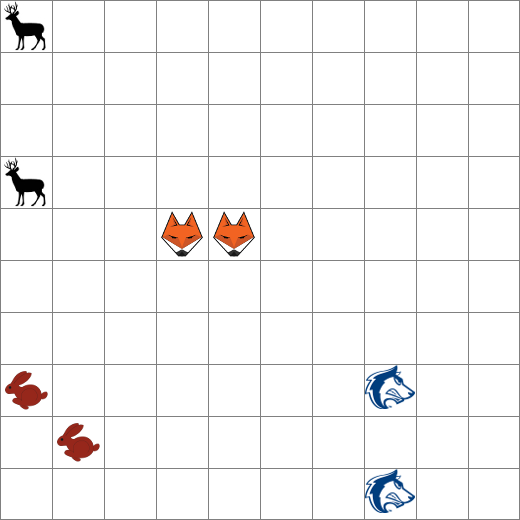
\includegraphics[scale=.65]{init.png}
	\caption{Initial state of animals}
	\label{fig:initialState}
	\end{figure}
}

{
	\begin{figure}[p]
	\centering
	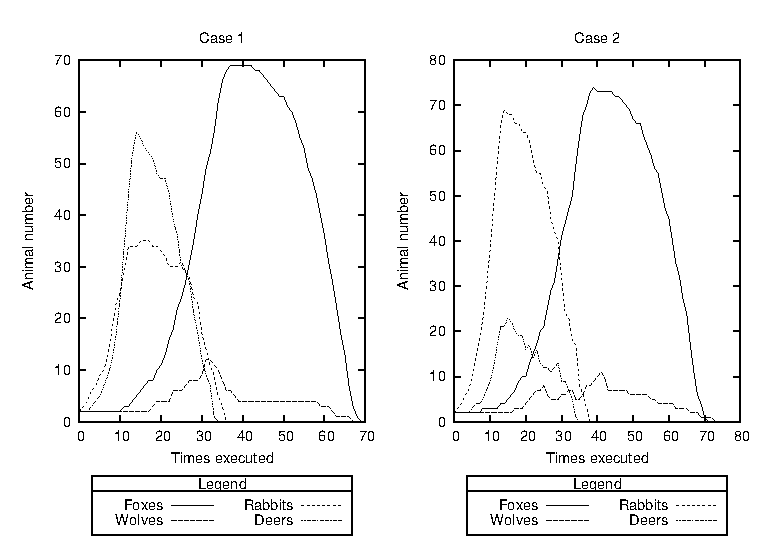
\includegraphics{plots.eps}
	\caption{The Behaviour of the animals}
	\label{fig:animalBehaviour}
	\end{figure}
}

{
	\begin{table}[p]
	\caption{Procreation of animals}

	\resizebox{8cm}{!} {
		\begin{tabular}{| c | c | c || c | c |}
		\hline

		 &\multicolumn{2}{|c||}{Predator} & \multicolumn{2}{c|}{Prey} \\
		\hline
		Case & Fox & Wolf & Rabbit & Deer \\
		\hline
		1 & 68 & 15 & 57 & 86 \\
		\hline
		2 & 90 & 0 & 90 & 54 \\
		\hline
		3 & 67 & 17 & 130 & 0 \\
		\hline
		4 & 84 & 0 & 131 & 0 \\
		\hline
		5 & 70 & 11 & 123 & 0 \\
		\hline
		6 & 82 & 0 & 88 & 45 \\
		\hline
		7 & 57 & 33 & 140 & 0 \\
		\hline
		8 & 80 & 11 & 135 & 0 \\
		\hline
		9 & 62 & 20 & 137 & 0 \\
		\hline
		10 & 90 & 0 & 70 & 72 \\
		\hline
		\end{tabular}
	}
	\label{tab:procreationTable}
	\centering
	\end{table}
}
\newpage
\end{document}


